\subsection{Grundlegende binomische Formeln}
\label{subsec:fundamentals_basic_binomial_formulas}

Die drei grundlegenden binomischen Formeln werden häufig verwendet, um
quadratische Terme umzuformen und Rechnungen zu vereinfachen.

Alle drei Formeln folgen direkt aus dem Distributivgesetz:

\subsubsection{Erste binomische Formel}
\label{subsubsec:fundamentals_first_binomial_formula}

Zunächst wird das Quadrat als Produkt geschrieben und ausmultipliziert:
\begin{align*}
  (a+b)^2
    &=(a+b)(a+b) \\
    &=a^2+ab+ba+b^2 \\
    &=a^2+2ab+b^2.
\end{align*}

\begin{TheoremBox}{Erste binomische Formel}{fundamentals_first_binomial_formula}
  \begin{ClozeArea}[\linewidth]{1.5cm}
    \[
      (a+b)^2=a^2+2ab+b^2.
    \]
  \end{ClozeArea}
\end{TheoremBox}

Die erste binomische Formel lässt sich auch geometrisch motivieren. Ein
Quadrat mit der Seitenlänge $a+b$ zerfällt in ein Quadrat der Fläche $a^2$,
zwei Rechtecke der Fläche $ab$ und ein Quadrat der Fläche $b^2$. Somit gilt
auch für die Flächen
\[
  (a+b)^2=a^2+ab+ab+b^2=a^2+2ab+b^2.
\]
\begin{center}
  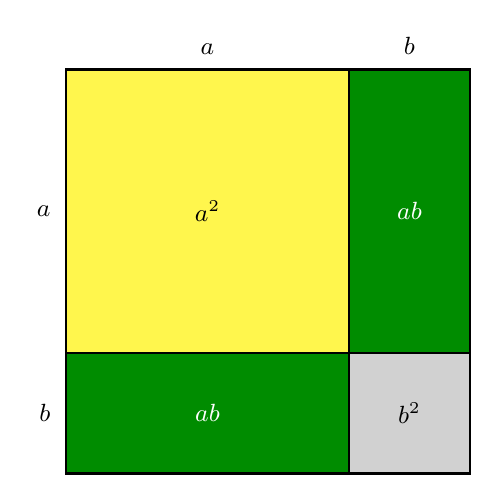
\begin{tikzpicture}[x=0.9cm,y=0.9cm,font=\small]
  \def\aside{4}
  \def\bside{1.7}
  \pgfmathsetmacro{\totalside}{\aside+\bside}

  \fill[yellow!70] (0,\bside) rectangle (\aside,\totalside);
  \fill[green!55!black] (\aside,\bside) rectangle (\totalside,\totalside);
  \fill[green!55!black] (0,0) rectangle (\aside,\bside);
  \fill[black!18] (\aside,0) rectangle (\totalside,\bside);

  \draw[thick] (0,0) rectangle (\totalside,\totalside);
  \draw[thick] (\aside,0) -- (\aside,\totalside);
  \draw[thick] (0,\bside) -- (\totalside,\bside);

  \node at ({0.5*\aside},{\bside+0.5*\aside}) {$a^2$};
  \node[text=white] at ({\aside+0.5*\bside},{\bside+0.5*\aside}) {$ab$};
  \node[text=white] at ({0.5*\aside},{0.5*\bside}) {$ab$};
  \node at ({\aside+0.5*\bside},{0.5*\bside}) {$b^2$};

  \node[above=2pt] at ({0.5*\aside},\totalside) {$a$};
  \node[above=2pt] at ({\aside+0.5*\bside},\totalside) {$b$};

  \node[left=2pt] at (0,{\bside+0.5*\aside}) {$a$};
  \node[left=2pt] at (0,{0.5*\bside}) {$b$};
\end{tikzpicture}

\end{center}

\subsubsection{Zweite binomische Formel}
\label{subsubsec:fundamentals_second_binomial_formula}

Auch hier wird zunächst ausmultipliziert und anschließend zusammengefasst:
\begin{align*}
  (a-b)^2
    &=(a-b)(a-b) \\
    &=a^2-ab-ba+b^2 \\
    &=a^2-2ab+b^2.
\end{align*}

\begin{TheoremBox}{Zweite binomische Formel}{fundamentals_second_binomial_formula}
  \begin{ClozeArea}[\linewidth]{1.5cm}
    \[
      (a-b)^2=a^2-2ab+b^2.
    \]
  \end{ClozeArea}
\end{TheoremBox}

\subsubsection{Dritte binomische Formel}
\label{subsubsec:fundamentals_third_binomial_formula}

Beim Produkt aus Summe und Differenz heben sich die gemischten Terme
gegenseitig auf:
\begin{align*}
  (a-b)(a+b)
    &=a^2+ab-ba-b^2 \\
    &=a^2-b^2.
\end{align*}

\begin{TheoremBox}{Dritte binomische Formel}{fundamentals_third_binomial_formula}
  \begin{ClozeArea}[\linewidth]{1.5cm}
    \[
      a^2-b^2=(a-b)(a+b).
    \]
  \end{ClozeArea}
\end{TheoremBox}

\begin{ExampleBox}{Binomische Formeln}{fundamentals_basic_binomial_formulas_example}
  \begin{enumerate}[label=(\alph*),itemsep=0.9em]
    \item
      \[
        (x+5)^2=\Cloze{7cm}{x^2+10x+25}.
      \]
    \item
      \[
        (3y-4)^2=\Cloze{7cm}{9y^2-24y+16}.
      \]
    \item
      \[
        (2a+3b)^2=\Cloze{8cm}{4a^2+12ab+9b^2}.
      \]
    \item
      \[
        4002^2-3998^2
        =\Cloze{10cm}{(4002-3998)(4002+3998)
          =4\cdot8000=32000}.
      \]
  \end{enumerate}
\end{ExampleBox}

\noindent\begin{minipage}{\linewidth}
\begin{DefinitionBox}{Quadratische Ergänzung}{fundamentals_completing_the_square}
  Bei der \emph{quadratischen Ergänzung} \EnglishTerm{completing the square}
  wird ein quadratischer Term so ergänzt, dass ein Binom nach der ersten oder
  zweiten binomischen Formel entsteht. Der ergänzte Wert wird gleichzeitig
  wieder subtrahiert, damit sich der Wert des Terms nicht ändert.
\end{DefinitionBox}

\begin{ExampleBox}{Quadratische Ergänzung}{fundamentals_completing_the_square_example}
  Der Term $x^2-2x+5$ enthält zunächst kein vollständiges Binom. Durch
  Ergänzen von $1$ erhält man
  \begin{ClozeArea}[\linewidth]{2.5cm}
    \begin{align*}
      x^2-2x+5
        &=x^2-2x+1-1+5 \\
        &=(x-1)^2+4.
    \end{align*}
  \end{ClozeArea}
\end{ExampleBox}
\end{minipage}
